\documentclass{article}
\usepackage{subfiles}
\usepackage{graphicx}
\usepackage{fancyhdr}
\usepackage{tabularx}
\usepackage{listings}
\usepackage[french]{babel}

\pagestyle{fancy}
\fancyhf{} % Efface les en-têtes et pieds de page par défaut
\fancyfoot[R]{\thepage} % Aligne le numéro de page à droite en bas
\renewcommand{\headrulewidth}{0pt} % Supprime la ligne en haut de page
\renewcommand{\footrulewidth}{0pt} % Supprime la ligne en bas de page

\begin{document}

\title{Document de conception \\ SAE S4.Deploi.01}
\author{Tristan Petit, Nils Hubert, Toni Rey,\\ 
 Majd El Sebeiti , Vianney Miquel}
\date{\today}
\maketitle
\begin{center}
    \vspace{1cm} % Espace entre la date et l'image
    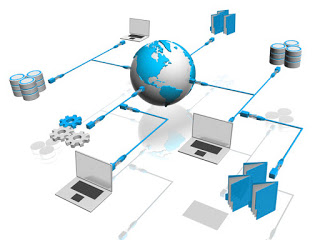
\includegraphics{Images/Logo-project.jpeg} % Ajuste le chemin et la taille
\end{center}

\maketitle

\pagenumbering{gobble}
\newpage
%nom de la table des matières
\renewcommand{\contentsname}{Table des matières}

%déclaration de la table des matières
\tableofcontents

\newpage
\pagenumbering{arabic}

\section{Introduction}

\subfile{Introduction/introduction.tex}

\section{Rappel et évolution sur l'architecture}

\subfile{architecture.tex}

\section{Ressources utilisées}

Pour notre SAE nous avons réunis les machines dans un cluster pour interconnecter nos hyperviseurs et de mutualiser les ressources qui sont répartis à travers nos hyperviseurs.

\begin{figure}[h]
    \centering
    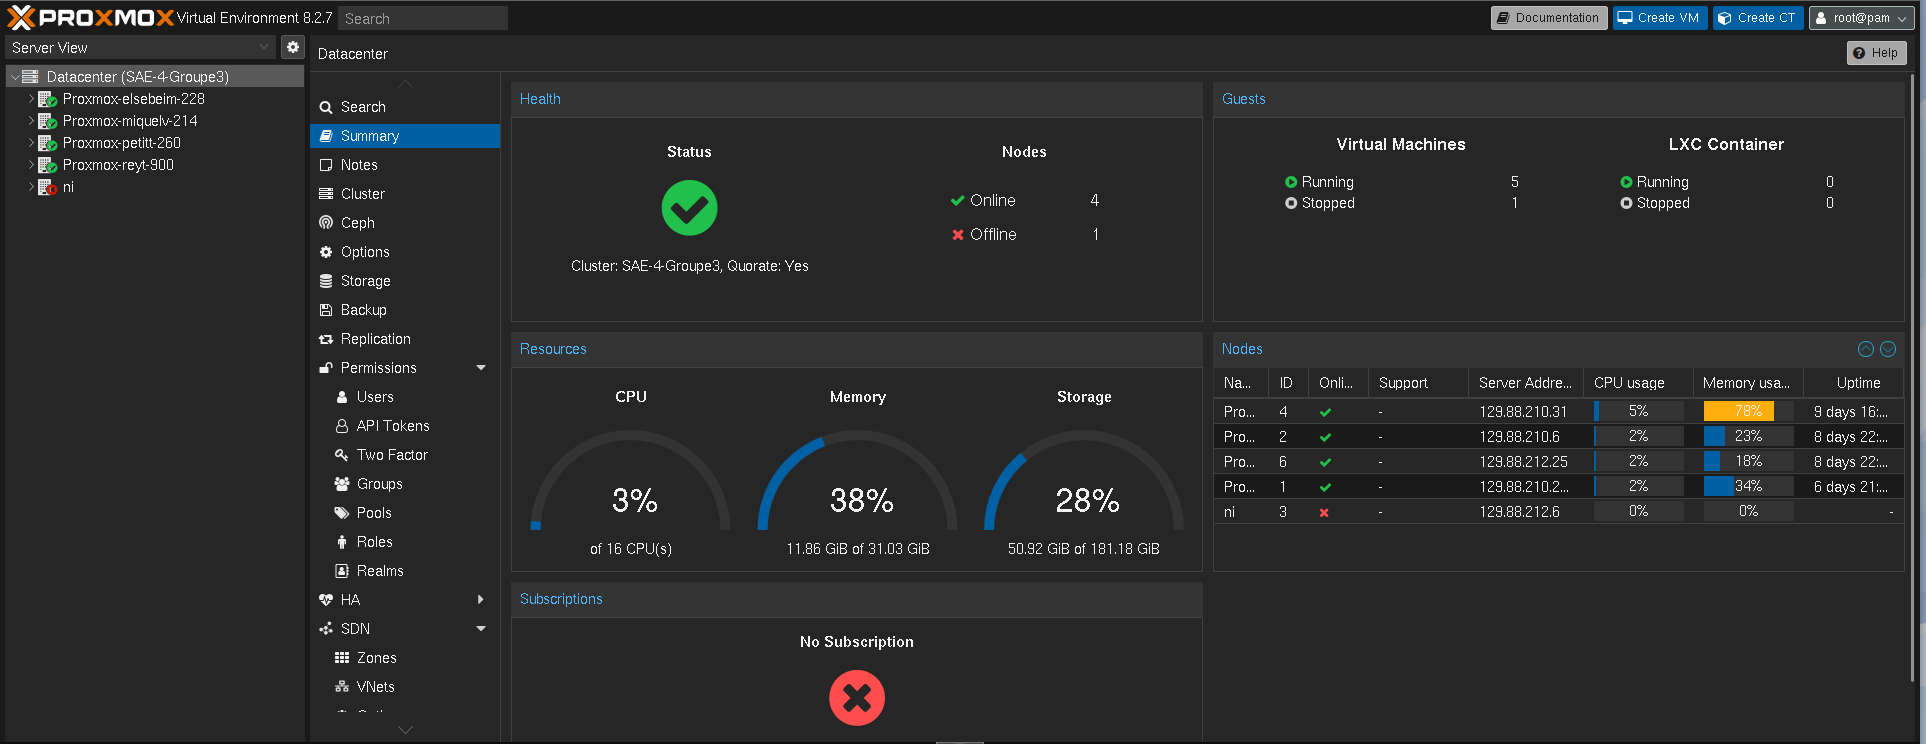
\includegraphics[width=1\textwidth]{Images/Ressource.png}
    \caption{Ressource utilisée pour la SAE sous proxmox}
    \label{fig:solution1}
\end{figure}

L'avantage de cette configuration par rapport à celle présente sur ASSR, c'est que nous n'avons pas machine virtuelle imbriqué
cela permet d'améliorer de manière significative les performances. \\
Le CPU est la ressource qui pose le moins de problème dans notre cas, il en est tout autre pour la RAM.
Celle ci va devoir être géré de manière équitable entre les hyperviseurs pour eviter une surcharge.
Le stockage ne devrait pas poser problème outre mesure, mais pourrait le devenir si l'on était dans l'obligation de rajouter 
des machines.

\section{Documentation Technique}

\subfile{DocTechnique/DNS/DNS.tex}
%\subfile{DocTechnique/routeurs/routeurs.tex}

\end{document}